% $HeadURL$

%%%%%%%%%%%%%%%%%%%%%%%%%%%%%%%%%%%%%%%%%%%%%%%%%%%%%%%%%%%%%%%%%%%%%%
%%                     Subunit
%%%%%%%%%%%%%%%%%%%%%%%%%%%%%%%%%%%%%%%%%%%%%%%%%%%%%%%%%%%%%%%%%%%%%%

\subsection{Glyphs: \glyph{Subunits}}
\label{sec:subunit}


\glyphContainer
Each \glyph{subunit} is represented by its own shape depending on its bio-molecular nature, as shown in \tab{subunit_containers}.
Those shapes are the same as those used to represent entity pools~(\sect{EPNs}).

% 


X[c,m]X[c,m]X[c,m]X[c,m]
    \toprule
    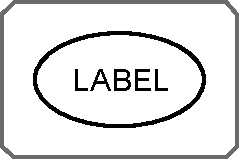
\includegraphics[scale = 0.8, valign = m]{images/unspecified-subunit} & 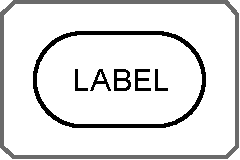
\includegraphics[scale = 0.8, valign = m]{images/simple_chemical-subunit} & 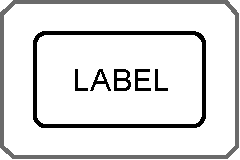
\includegraphics[scale = 0.8, valign = m]{images/macromolecule-subunit} & 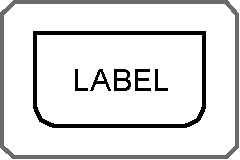
\includegraphics[scale = 0.8, valign = m]{images/genetic-subunit}\\[0.2cm]
    \glyph{unspecified entity subunit} & \glyph{simple chemical subunit} & \glyph{macromolecule subunit} & \glyph{nucleic acid feature subunit}\\[0.5cm]
    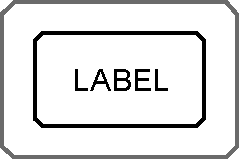
\includegraphics[scale = 0.8, valign = m]{images/complex-subunit} & 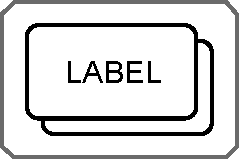
\includegraphics[scale = 0.8, valign = m]{images/macromolecule-multimer-subunit} & 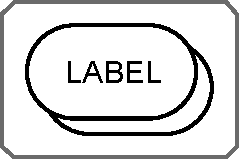
\includegraphics[scale = 0.8, valign = m]{images/simple_chemical-multimer-subunit} & 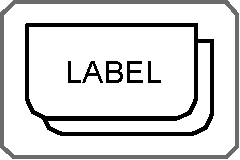
\includegraphics[scale = 0.8, valign = m]{images/genetic-multimer-subunit}\\[0.2cm]
    \glyph{complex subunit} & \glyph{multimer of macromolecules subunit} & \glyph{multimer of simple chemicals subunit} & \glyph{multimer of nucleic acid feature subunit}\\[0.5cm]
    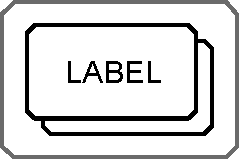
\includegraphics[scale = 0.8, valign = m]{images/complex-multimer-subunit} &  &  & \\[0.2cm]
    \glyph{multimer of complexes subunit} & & & \\
    \bottomrule
\end{tabu}
\caption{The \PD glyphs for the different types of \glyph{subunits}.
Each \glyph{subunit} decorates a \glyph{complex}.}
\label{tab:subunit_containers}
\end{table}


\begin{figure}[htb]
  \centering
  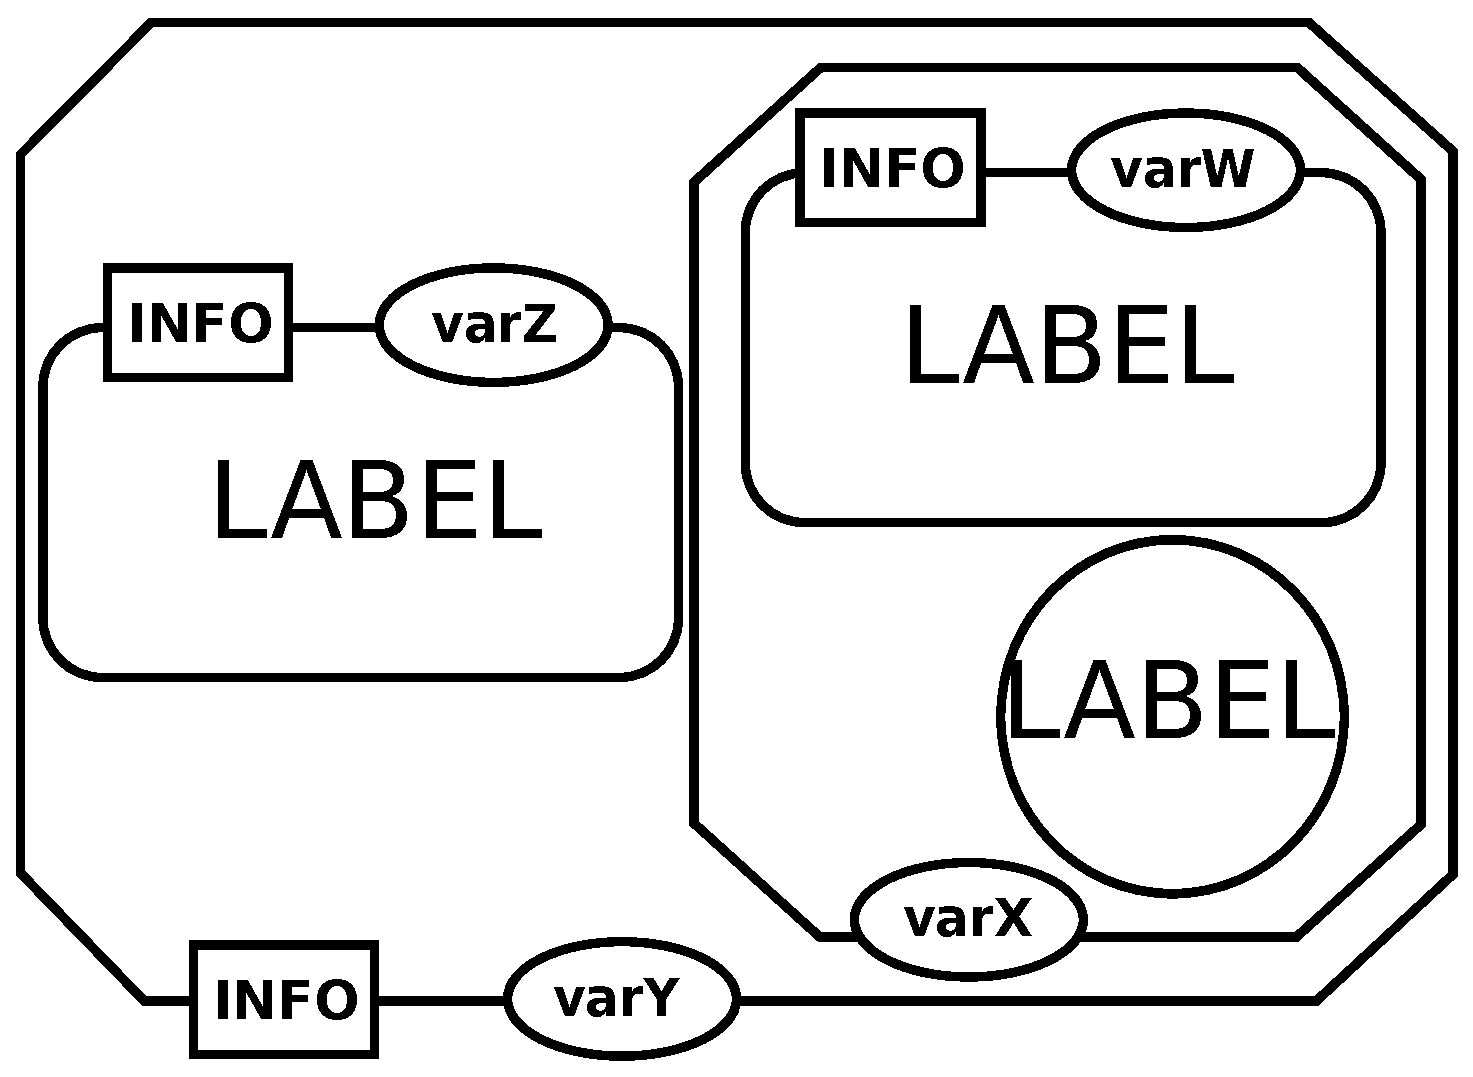
\includegraphics[scale=0.8]{images/complex}
  \caption{Both these complex glyphs are equivalent.
      The complex on the left is described using \glyph{subunit} decorators.
      The complex on the right depicts the same information, without explicitly representing those subunits, that are only suggested by the label of the \glyph{complex}.
  However, their states are represented using \glyph{state variables} decorating the \glyph{complex}.}
  \label{fig:complexSubunits}
\end{figure}


